\subsection{Vakken - FR2} 

%Ingeschreven vakken bekijken  
\subsubsection{Ingeschreven vakken bekijken}      
\noindent\begin{table}[H]
            \begin{tabular}{l | p{10cm}}
                \textbf{ID:} & FR2.1 \\ \hline
                \textbf{TITEL:} & Ingeschreven vakken bekijken\\ \hline
                \textbf{PRIORITEIT:} &  Hoog \\ \hline
                \textbf{PREREQUISITIES:} & \\ \hline
                \textbf{TOEGANG:} &  Student \\ \hline
                \textbf{BESCHRIJVING:} & Een aangemelde student kan ten alle tijden de lijst van vakken zien waarvoor deze is ingeschreven. De student drukt hiervoor op een knop getiteld “Ingeschreven Vakken” en wordt dan naar een pagina doorgestuurd waarop deze in lijstvorm te zien zijn.\\
            \end{tabular}\\
            \caption{FR2.1 - Ingeschreven vakken bekijken}
            \label{tab:FR2.1 - Ingeschreven vakken bekijken}
        \end{table}  
        
\textbf{Stappenplan:}
	\begin{enumerate}
	\item Aangemelde student ziet zijn persoonlijke hoofdpagina (zie figuur \ref{fig:CalZone Profile}) en kan bovenaan op de optie "Ingeschreven Vakken" klikken.
	\item Gebruiker klikt op de knop 'Ingeschreven Vakken'
	\item Gebruiker krijgt overzicht van alle ingeschreven vakken (zie figuur \ref{fig:CalZone Enrolled})
	\end{enumerate}

\begin{center}
\begin{figure}[H]
\caption{CalZone Enrolled}
\centerline{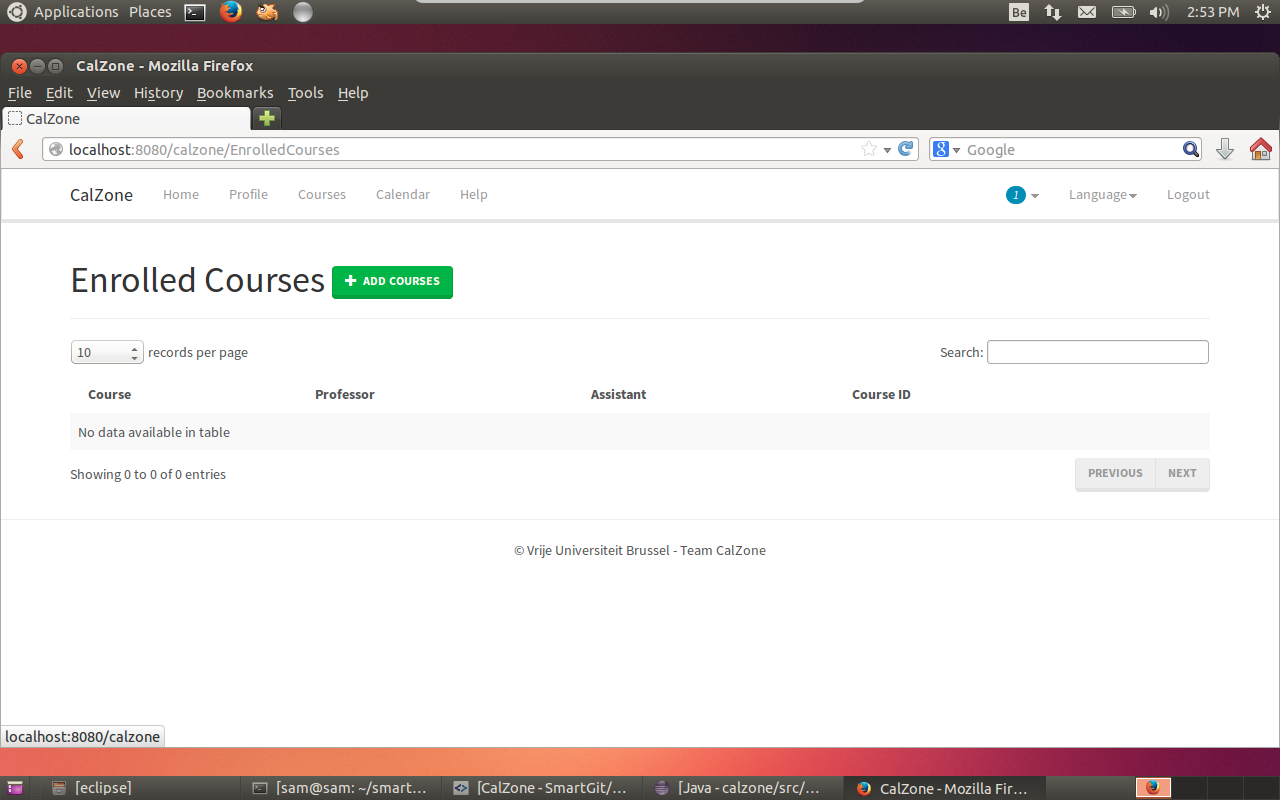
\includegraphics[scale=0.4]{img/CalzoneEnrolled}}
\label{fig:CalZone Enrolled}
\end{figure}
\end{center}

%Notificaties van last-minute verandering krijgen
\subsubsection{Notificaties van last-minute verandering krijgen}        
\noindent\begin{table}[H]
            \begin{tabular}{l | p{10cm}}
                \textbf{ID:} & FR2.2 \\ \hline
                \textbf{TITEL:} & Notificaties van last-minute veranderingen \\ \hline
                \textbf{PRIORITEIT:} &  Medium \\ \hline
                \textbf{PREREQUISITIES:} & \\ \hline
                \textbf{TOEGANG:} & Student, Assistent, Professor \\ \hline
                \textbf{BESCHRIJVING:} & Mocht er een lesaanpassing plaats vinden (bijv.: een professor die de les van lokaal verandert) dan moeten de gebruiker die dat vak volgen of geven verwittigd worden. Zij zullen dan een bericht op hun e-mail adres ontvangen met daarin de nodige informatie over de lesaanpassing.\\
            \end{tabular}\\
            \caption{FR2.2 - Notificaties van last-minute veranderingen}
			\label{tab:FR2.2 - Notificaties van last-minute veranderingen}
        \end{table}      
        
\textbf{Stappenplan:}
	\begin{enumerate}
	\item Een les uur of locatie word aangepast in het systeem. Als deze les de zelfde dag nog word gegeven zal er een last minute notificatie worden verzonden.
	\item Het programma kijkt naar iedereen die deze les volgt en zend een email naar het geassocieerde vub adres.
	\item De betreffende gebruikers krijgen dan een notificatie op hun hoofdpagina te zien (zie figuur \ref{fig:CalZone Notification}).
	\item Optioneel: Ingelogde gebruikers krijgen een browser notificatie dat er een aanpassing is gedaan aan het programma.  
	\end{enumerate}
	
\begin{center}
\begin{figure}[H]
\caption{CalZone Notification}
\centerline{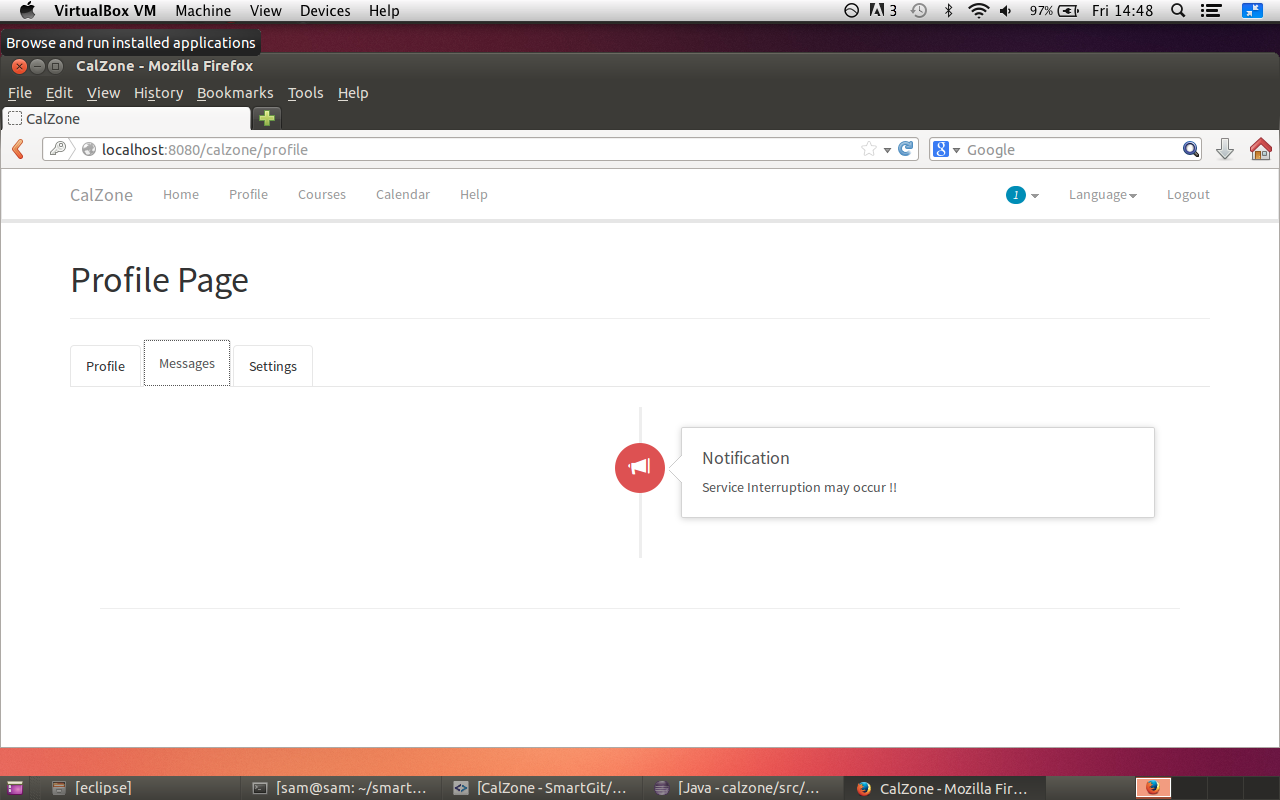
\includegraphics[scale=0.4]{img/CalzoneNotification}}
\label{fig:CalZone Notification}
\end{figure}
\end{center}

%Last-minute tijdstip vak aanpassen
\subsubsection{Last-minute tijdstip vak aanpassen} 
\noindent\begin{table}[H]
            \begin{tabular}{l | p{10cm}}
                \textbf{ID:} & FR2.3 \\ \hline
                \textbf{TITEL:} & Last-minute tijdstip vak aanpassen\\ \hline
                \textbf{PRIORITEIT:} &  Medium \\ \hline
                \textbf{PREREQUISITIES:} & \\ \hline
                \textbf{TOEGANG:} & Assistent, Professor \\ \hline
                \textbf{BESCHRIJVING:} & Een gebruiker (van type toegang) heeft de optie om het tijdstip van een vak last-minute aan te passen. Enkel toegelaten als deze gebruiker de les zelf geeft of de programmabeheerder is.  De gebruiker drukt dan op de knop getiteld “Lesuur aanpassen” en wordt dan gevraagd om een nieuwe dag en een tijdstip uit te kiezen. 
                                        Hierna wordt dan een e-mail gestuurd naar alle studenten die dat vak volgen met het nieuwe tijdstip van het vak.\\ 
            \end{tabular}\\
            \caption{FR2.3 - Last-minute tijdstip vak aanpassen}
            \label{tab:FR2.3 - Last-minute tijdstip vak aanpassen}
        \end{table}
       
\textbf{Stappenplan:}
	\begin{enumerate}
	\item Gebruiker vertrekt vanuit zijn persoonlijke hoofdpagina (zie figuur \ref{fig:CalZone Profile}).
	\item Gebruiker selecteer de les die hij wil aanpassen
	\item Met de juiste les geselecteerd klikt de gebruiker op 'Last-Minute aanpassing'. Dit gaat enkel 48 uur voor het starten van de les
	\item Het is dan mogelijk om voor de gebruiker een nieuw uur te selecteren.
	\item Gebruiker kan dan op 'toepassen' klikken waarop een conflictdetectie kan gebeuren.
	\item Eventuele conflicten worden aangeduid waarop de gebruiker moet beslissen of hij al dan niet de aanpassing wilt doen
	\end{enumerate}
        
%Locatie Les aanpassen
\subsubsection{Locatie Les aanpassen} 
\noindent\begin{table}[H]
            \begin{tabular}{l | p{10cm}}
                \textbf{ID:} & FR2.4 \\ \hline
                \textbf{TITEL:} & Locatie les aanpasen\\ \hline
                \textbf{PRIORITEIT:} &  Medium \\ \hline
                \textbf{PREREQUISITIES:} & \\ \hline
                \textbf{TOEGANG:} & Assistent, Professor \\ \hline
                \textbf{BESCHRIJVING:} & Een professor heeft de optie om de locatie van een vak aan te passen. 
                                        De professor drukt dan op de knop getiteld “Lokaal aanpassen” en wordt dan gevraagd om een nieuwe locatie uit te kiezen, deze locatie is dan van de vorm G.V.L (met G = gebouw, V = verdieping en L = lokaal). De Scheduler zal dan nagaan of het ingevoerde lokaal vrij is op het tijdstip van het vak. Keurt de Scheduler het nieuwe lokaal goed, dan wordt er een e-mail gestuurd naar alle studenten die het vak volgen met daarin het nieuwe lokaal van het vak. Keurt de Scheduler het nieuwe lokaal af, dan wordt de professor gevraagd een ander lokaal in te geven.\\ 
            \end{tabular}\\
            \caption{FR2.4 - Locatie les aanpassen}
            \label{tab:FR2.4 - Locatie les aanpassen}
        \end{table}
        
\textbf{Stappenplan:}
	\begin{enumerate}
	\item Gebruiker vertrekt vanuit zijn persoonlijke hoofdpagina (zie figuur \ref{fig:CalZone Profile}).
	\item Gebruiker selecteer les dat hij wilt aanpassen
	\item Met de juiste les geselecteerd klikt de gebruiker op 'Last-Minute aanpassing'. Dit gaat enkel 48 uur voor het starten van de les
	\item Het is dan mogelijk om voor de gebruiker een nieuw lokaal te selecteren.
	\item Gebruiker krijgt de optie om eerst gebouw te kiezen. Vervolgens de verdieping en dan het lokaal. Dit om te voorkomen dat er lokalen worden geselecteerd die niet bestaan.
	\item Gebruiker kan dan op 'toepassen' klikken waarop een conflictdetectie kan gebeuren.
	\item Eventuele conflicten worden aangeduid waarop de gebruiker moet beslissen of hij al dan niet de aanpassing wilt doen 
	\item Optioneel: Selecteer vak dat ervoor zorgt dat het enkel mogelijk is lokalen te selecteren waar geen lessen gegeven worden.
	\end{enumerate}	        
        
        
%Details les aanpassen 
\subsubsection{Details les aanpassen} 
\noindent\begin{table}[H]
            \begin{tabular}{l | p{10cm}}
                \textbf{ID:} & FR2.5 \\ \hline
                \textbf{TITEL:} & Details vak aanpassen\\ \hline
                \textbf{PRIORITEIT:} &  Laag \\ \hline
                \textbf{PREREQUISITIES:} & \\ \hline
                \textbf{TOEGANG:} & Professor, Programmabeheerder \\ \hline
                \textbf{BESCHRIJVING:} & Een professor kan de beschrijving en details van een vak aanpassen. Hiervoor zal er een knop getiteld “Aanpassen” zijn, waarna de professor vrij is in het aanpassen van de details. \\ 
            \end{tabular}\\
            \caption{FR2.5 - Details vak aanpassen}
            \label{tab:FR2.5 - Details vak aanpassen}
        \end{table}	
        
\textbf{Stappenplan:}
	\begin{enumerate}
	\item De gebruiker vertrekt vanuit zijn persoonlijke hoofdpagina (zie figuur \ref{fig:CalZone Profile}). De gebruiker gaat naar zijn gebruikersprofiel via de knop bovenaan op het scherm.
	\item De gebruiker klikt vervolgens op 'Vakken' en krijgt hierbij een overzicht van de vakken waaraan hij gekoppeld is.
	\item De gebruiker kan dan op de knop 'Aanpassen' klikken ter hoogte van het gewenste vak.
	\item Gebruiker krijgt dan de opties om het detailformulier aan te passen van het vak.
	\item Gebruiker kan vervolgens op 'Opslaan' klikken.
	\end{enumerate}

\textbf{Opmerking:}
	\begin{enumerate}
	\item Vak details moeten worden aangepast voor runnen van een scheduler. Als er aanpassingen moeten gebeuren nadien, zoals meer lessen HOC. Moet dit rechtstreeks en manueel verlopen via de programmabeheerder.
	\end{enumerate}
        
%Detail formulier nieuw vak indienen
\subsubsection{Detail formulier nieuw vak indienen} 
\noindent\begin{table}[H]
            \begin{tabular}{l | p{10cm}} 
                \textbf{ID:} & FR2.6 \\ \hline
                \textbf{TITEL:} & Detail formulier nieuw vak indienen\\ \hline
                \textbf{PRIORITEIT:} &  Laag \\ \hline
                \textbf{PREREQUISITIES:} & \\ \hline
                \textbf{TOEGANG:} & Professor \\ \hline
                \textbf{BESCHRIJVING:} & Mocht er nood zijn aan het toevoegen van een nieuw vak aan de database, dan kan een professor hiervoor een formulier opstellen met daarin:
        \begin{itemize}\itemsep1pt \parskip0pt \parsep0pt
                                        \item beschrijving van het vak
                                        \item aantal studiepunten
                                        \item nodige prerequisities
                                        \item welk semester het vak gegeven wordt
                                        \item aantal uren studie tijd
                                        \item studiegidsnummer
                                        \item 2e zittijd mogelijk
                                        \item onderwijstaal
                                        \item faculteit
                                        \item verantwoordelijke vakgroep
                                        \item onderwijsteam
                                        \item onderdelen en contacturen
                                        \item studiemateriaal
                                        \item leerresultaten
                                        \item beoordelingsinformatie
                                        \end{itemize}
                                        Het formulier wordt dan gestuurd naar de Programmabeheerder die het vak zal toevoegen. 
            \end{tabular}\\
            \caption{FR2.6- Detail formulier nieuw vak indienen}
            \label{tab:FR2.6 - Detail formulier nieuw vak indienen}
        \end{table}
        
\textbf{Stappenplan:}
	\begin{enumerate}
	\item  De gebruiker vertrekt vanuit zijn persoonlijke hoofdpagina (zie figuur \ref{fig:CalZone Profile}). De gebruiker gaat naar zijn gebruikersprofiel via de knop bovenaan op het scherm.
	\item De gebruiker klikt vervolgens op 'Vakken' en krijgt hierbij een overzicht van de vakken waaraan hij gekoppeld is.
	\item De gebruiker kan dan op de knop 'Toevoegen' klikken ter hoogte van het gewenste vak.
	\item Gebruiker krijgt nu een formulier voor een nieuw vak aan te maken (zie figuur \ref{fig:CalZone New Course}).
	\item Na het invullen kan de gebruiker op 'Indienen' klikken.
	\item Hierbij word eerst controle gedaan of de informatie voldoende ingevuld is. Als dit zo is gaan we naar de volgende stap. Als er error in het formulier zitten krijgt de gebruiker een error toegewezen om het veld dat voor problemen zorgt. Hij kan dit nu aanpassen en weer op 'Indienen' klikken.
	\item Een ingediend detail formulier moet goedgekeurd worden door de programmabeheerder om zo in het systeem te komen.
	\end{enumerate}
	
\begin{center}
\begin{figure}[H]
\caption{CalZone New Course}
\centerline{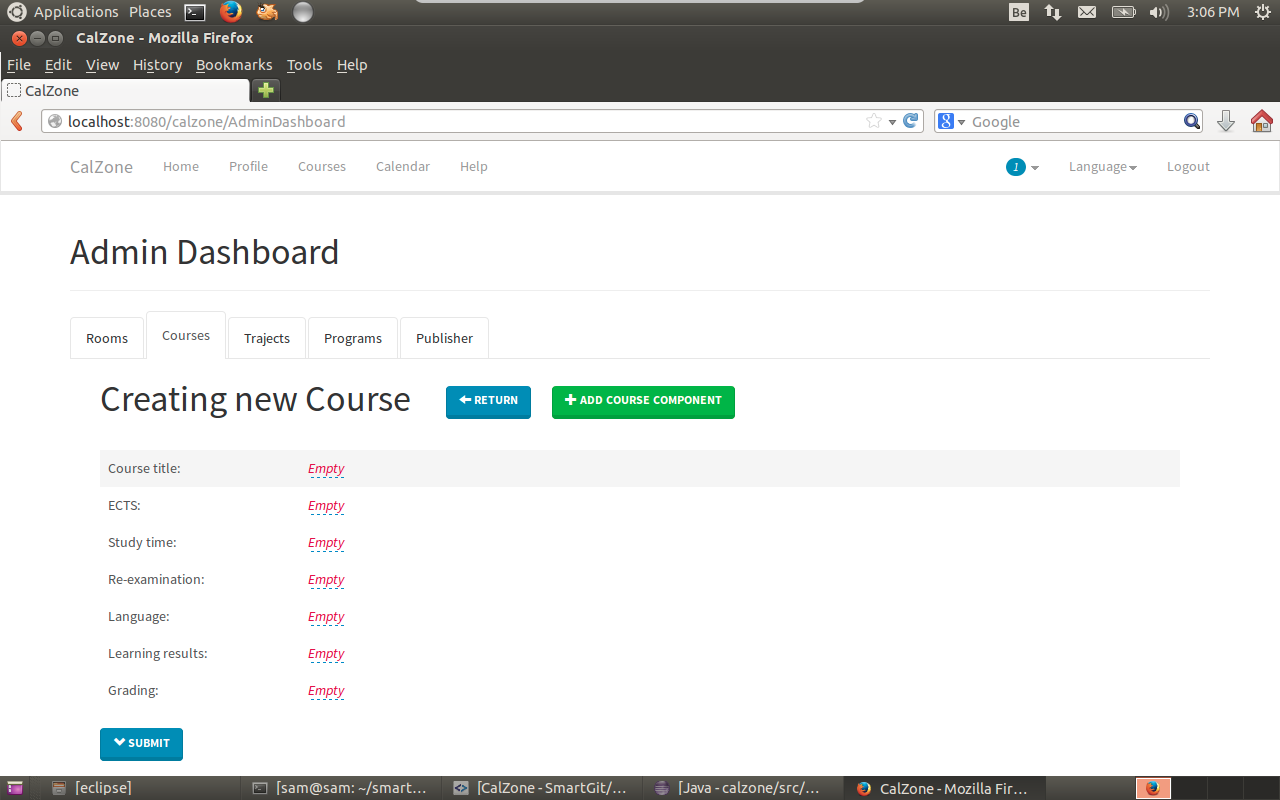
\includegraphics[scale=0.4]{img/CalzoneAdminNewCourse}}
\label{fig:CalZone New Course}
\end{figure}
\end{center}

%Goedkeuren detail formulier 
\subsubsection{Goedkeuren detail formulier}     
\noindent\begin{table}[H]
            \begin{tabular}{l | p{10cm}}
                \textbf{ID:} & FR2.7 \\ \hline
                \textbf{TITEL:} & Goedkeuren detail formulier   \\ \hline
                \textbf{PRIORITEIT:} &  Laag \\ \hline
                \textbf{PREREQUISITIES:} & De professor moet al een detail formulier ingedient hebben\\ \hline
                \textbf{TOEGANG:} & Programmabeheerder \\ \hline
                \textbf{BESCHRIJVING:} & De programma beheerder bekijkt en ingediende formulier van een professor en beslist dit toe wel of niet toe te voegen aan het de database. 
            \end{tabular}\\
            \caption{FR2.7 - Goedkeuren detail formulier  }
            \label{tab:FR2.7 - Goedkeuren detail formulier  }
        \end{table}
 
\textbf{Stappenplan:}
	\begin{enumerate}
	\item De gebruiker vertrekt vanuit zijn persoonlijke hoofdpagina (zie figuur \ref{fig:CalZone Profile}). De gebruiker gaat naar zijn gebruikersprofiel via de knop bovenaan op het scherm.
	\item De gebruiker klikt vervolgens op 'Vakken' en krijgt hierbij een overzicht van de vakken waaraan hij gekoppeld is.
	\item De gebruiker kan dan op de knop 'Wachtende Vakken' klikken.
	\item Gebruiker krijgt nu een formulier voor een nieuw vak met de informatie die de professor heeft ingegeven.
	\item Na het invullen kan de gebruiker op 'Goedkeuren' of 'Afkeuren' drukken
		\begin{enumerate}
		\item Als een formulier word afgekeurd word het verwijderd en krijgt de desbetreffende professor een notificatie in zijn mailbox.
		\item Als een formulier word goedgekeurd word deze toegevoegd aan de database van vakken en krijgt de desbetreffende professor een notificatie in zijn mailbox.
		\end{enumerate}
	\end{enumerate}       
         
%Planning markeren als voorstel 
\subsubsection{Planning markeren als voorstel}         
\noindent\begin{table}[H]
            \begin{tabular}{l | p{10cm}}
                \textbf{ID:} & FR2.8 \\ \hline
                \textbf{TITEL:} & Planning markeren als voorstel\\ \hline
                \textbf{PRIORITEIT:} &  Medium \\ \hline
                \textbf{PREREQUISITIES:} & \\ \hline
                \textbf{TOEGANG:} & Professor \\ \hline
                \textbf{BESCHRIJVING:} & Een professor kan een voorstel indienen aan de Scheduler. 
                                        Deze geeft dan in wanneer hij zijn vak het liefst zou geven en dan wordt dit doorgegeven aan de Scheduler die dan rekening probeert te houden met de ingegeven constraint. Dit staat los van de beschikbaarheid van de professor en lokalen.  \\
            \end{tabular}\\
            \caption{FR2.8 - Planning markeren als voorstel}
            \label{tab:FR2.8 - Planning markeren als voorstel}
        \end{table}
        
\textbf{Stappenplan:}
	\begin{enumerate}
	\item De gebruiker gaat naar zijn gebruikersprofiel via de knop recht op het scherm.
	\item De gebruiker klikt vervolgens op 'Vakken' en krijgt hierbij een overzicht van de vakken waaraan hij gekoppeld is.
	\item De gebruiker kan dan op de knop 'Toevoegen Voorstel' klikken ter hoogte van het gewenste vak.
	\item Gebruiker krijgt nu een formulier voor een nieuw voorstel in te dienen. Dit gebeurd door selectie les per les toe te voegen gebruik makende van volgende parameters.
		\begin{itemize}
		\item Dag v/d week (Verplicht)
		\item Begin uur (Verplicht)
		\item Eind uur (Verplicht)
		\item Lokaal (Optioneel)
		\item Herhaling: Eenmalig, x Weken
		\end{itemize}
	\item Het is mogelijk om verschillende van deze lessen in te geven door steeds op 'Toevoegen' te klikken en het proces hierboven te herhalen.
	\item Na het invullen van een of meerdere lessen kan de gebruiker op 'Indienen' klikken.
	\item Entrys verwijderen kan ook door op 'Delete' te klikken. Corresponderende met het entry veld.
	\item Hierbij word eerst controle gedaan of de informatie voldoende ingevuld is volgens het detailformulier van het vak. Bij een error kan de gebruiker deze nog proberen op te lossen en opnieuw op 'Indienen' klikken.
	\item Een ingediend formulier kan de scheduler gebruiken als het mogelijk is om aan het voorstel te voldoen.
	\end{enumerate}	        

%Vakken verwijderen van lesprogramma
\subsubsection{Vakken verwijderen van lesprogramma}        
\noindent\begin{table}[H]
            \begin{tabular}{l | p{10cm}}
                \textbf{ID:} & FR2.9 \\ \hline
                \textbf{TITEL:} & Vakken verwijderen van lesprogramma\\ \hline
                \textbf{PRIORITEIT:} &  Hoog \\ \hline
                \textbf{PREREQUISITIES:} & \\ \hline
                \textbf{TOEGANG:} & Programmabeheerder \\ \hline
                \textbf{BESCHRIJVING:} & De Programmabeheerder kan ook vakken verwijderen uit lesprogramma’s \\ 
            \end{tabular}\\
            \caption{FR2.9 - Vakken verwijderen van lesprogramma}
            \label{tab:FR2.9 - Vakken verwijderen van lesprogramma}
        \end{table}    
        
\textbf{Stappenplan:}
	\begin{enumerate}
	\item De gebruiker gaat naar zijn gebruikersprofiel via de knop recht op het scherm.
	\item De gebruiker klikt vervolgens op 'Vakken' en krijgt hierbij een overzicht van de vakken waaraan hij gekoppeld is. Bij de programmabeheerder zijn dit alle vakken in het systeem.
	\item De gebruiker kan vervolgens klikken op de knop 'Verwijderden' corresponderend met het juiste vak.
	\end{enumerate}	    
        
\clearpage